\documentclass[11pt,a4paper]{article}

\usepackage[margin=1in]{geometry}
\usepackage{hyperref}
\usepackage{xcolor}
\usepackage{listings}
\usepackage{graphicx}
\usepackage{amsmath}
\usepackage{amssymb}
\usepackage{booktabs}
\usepackage{array}
\usepackage{fancyhdr}
\usepackage{tikz}
\usetikzlibrary{shapes,arrows,positioning,decorations.pathmorphing}

% Define code style
\lstset{
    language=C++,
    basicstyle=\ttfamily\small,
    keywordstyle=\color{blue},
    commentstyle=\color{gray},
    stringstyle=\color{red},
    breaklines=true,
    showstringspaces=false,
    tabsize=2,
    numbers=left,
    numberstyle=\tiny,
    frame=single,
    backgroundcolor=\color{white}
}

\lstdefinelanguage{json}{
    basicstyle=\ttfamily\small,
    numbers=left,
    numberstyle=\tiny,
    stepnumber=1,
    numbersep=8pt,
    showstringspaces=false,
    breaklines=true,
    frame=lines,
    stringstyle=\color{red},
    identifierstyle=\color{black},
    keywordstyle=\color{blue},
}

\setlength{\headheight}{15pt}
\pagestyle{fancy}
\lhead{subFlow Library Documentation}
\rhead{\today}
\cfoot{\thepage}

\title{\textbf{subFlow Library Documentation}\\
A Lightweight C++ Framework for Multiphase Flow Simulation in Porous Media}
\author{Generated Documentation}
\date{\today}

\begin{document}

\maketitle

\tableofcontents
\newpage

\section{Introduction}

subFlow is a lightweight, modular C++ library designed for analyzing multiphase flow in porous media with three phases: water, oil, and gas. The library implements a coupled numerical scheme combining a locally conservative Darcy solver with a saturation transport solver to simulate phase displacement and transport in heterogeneous reservoirs.

\subsection{Key Features}

\begin{itemize}
    \item \textbf{Multiphase Formulation:} Water--oil--gas systems with flexible phase combinations
    \item \textbf{Darcy Flow Solver:} Compressible and incompressible options using locally conservative finite element formulation with $\mathbf{H}(\text{div})$--$L^2$ approximation pairs for total flux and pressure
    \item \textbf{Transport Solver:} Finite Volume scheme with robust upwinding, conservation properties, and gravitational segregation using Implicit Hybrid Upwind (IHU) strategy
    \item \textbf{Coupling Strategy:} Sequential Fully Implicit (SFI) method for handling strong nonlinear coupling between flow and transport
    \item \textbf{Flexible I/O:} Parameterized JSON-based input configuration and support for mesh files (.geo, .msh)
    \item \textbf{Modular Design:} Clear interfaces enabling extension and customization of physics, discretization, and coupling strategies
\end{itemize}

\subsection{Typical Workflow}

The standard workflow for simulating multiphase flow with subFlow consists of four main stages:

\begin{enumerate}
    \item \textbf{Mesh and Data Preparation:} Build or import the computational mesh and provide rock/fluid properties
    \item \textbf{Darcy Problem Solution:} Solve for pressure and total flux using $\mathbf{H}(\text{div})$--$L^2$ finite element method
    \item \textbf{Transport Advancement:} Advance saturation profiles using Finite Volume transport solver with proper flux handling
    \item \textbf{SFI Coupling:} Iterate until convergence for each time step using the Sequential Fully Implicit coupling scheme
\end{enumerate}

\newpage
\section{Preprocessing Classes}

Preprocessing classes handle the preparation of the computational problem, including reading input data, building meshes, and setting up the approximation spaces.

\subsection{TSFProblemData}

\textbf{Purpose:} Central data container that stores all information required to set up a reservoir problem.

\textbf{Location:} \lstinline|src/TSFProblemData.h|

\textbf{Responsibilities:}
\begin{itemize}
    \item Read and parse JSON configuration files containing simulation parameters
    \item Store geometric mesh information, domain properties, and boundary conditions
    \item Manage fluid properties (density, viscosity, compressibility models)
    \item Store rock properties (permeability, porosity) for each domain
    \item Manage numerical parameters (analysis type, time stepping, solver tolerances)
    \item Handle initial conditions (pressure and saturation profiles)
    \item Provide petro-physical parameters (relative permeability models, residual saturations)
\end{itemize}

\textbf{Key Methods:}
\begin{lstlisting}[language=C++]
// Read problem data from JSON file
void ReadJSONFile(std::string filename);

// Serialization methods for saving/loading state
void Write(TPZStream &buf, int withclassid) const;
void Read(TPZStream &buf, void *context);
\end{lstlisting}

\textbf{Data Structures:}

The class contains nested structures for organizing related data:

\begin{description}
    \item[\lstinline|TGeometry|] Stores mesh information including domain names, material IDs, mesh source (GMSH), and standard material IDs for various element types
    \item[\lstinline|TNumerics|] Contains numerical parameters: analysis type, time stepping, convergence tolerances, iteration limits, thread counts
    \item[\lstinline|TFluidProperties|] Fluid data: density, viscosity, compressibility models for water and gas
    \item[\lstinline|TPetroPhysics|] Rock properties: relative permeability model and residual saturations
    \item[\lstinline|TReservoirProperties|] Initial conditions for pressure and saturation
    \item[\lstinline|TPostProcess|] Output control: post-processing frequency, threading options, VTK resolution
\end{description}

\subsection{TSFApproxCreator}

\textbf{Purpose:} Builds the finite element approximation spaces and computational meshes for Darcy and transport problems.

\textbf{Location:} \lstinline|src/TSFApproxCreator.h|

\textbf{Responsibilities:}
\begin{itemize}
    \item Configure the Darcy finite element space ($\mathbf{H}(\text{div})$ for fluxes, $L^2$ for pressure)
    \item Create atomic computational meshes for different physical spaces
    \item Construct multiphysics computational mesh coupling flux and pressure spaces
    \item Add material objects for Darcy equation
    \item Condense high-order elements to improve computational efficiency
    \item Build auxiliary transport mesh for post-processing and interface identification
    \item Insert interface elements between subdomains
\end{itemize}

\textbf{Key Methods:}
\begin{lstlisting}[language=C++]
// Set problem data reference
void SetProblemData(TSFProblemData *simData);

// Configure Darcy approximation space
void ConfigureDarcySpace();

// Add Darcy materials to the mesh
void AddDarcyMaterials();

// Create complete approximation space (main driver)
TPZMultiphysicsCompMesh *CreateApproximationSpace();

// Condense elements for efficiency
void CondenseElements(TPZCompMesh *cmesh, 
                      char LagrangeLevelNotCondensed, 
                      bool keepmatrix = true);

// Build auxiliary transport mesh
void BuildTransportCmesh();

// Create interface elements
void CreateInterfaceElements();

// Get transport mesh reference
TPZCompMesh *GetTransportCmesh();
\end{lstlisting}

\subsection{TPZFastCondensedElement}

\textbf{Purpose:} Implements static condensation of high-order element degrees of freedom to reduce the system size.

\textbf{Location:} \lstinline|src/TPZFastCondensedElement.h|

\textbf{Responsibilities:}
\begin{itemize}
    \item Perform element-level static condensation (Schur complement)
    \item Eliminate interior degrees of freedom without solving the full system
    \item Improve computational efficiency for high-order approximations
    \item Maintain matrix structure for efficient storage and assembly
\end{itemize}

\newpage
\section{Input File Format}

subFlow uses JSON-based configuration files to define simulation parameters. This section describes the structure and available options.

\subsection{JSON File Structure Overview}

A complete subFlow configuration file contains six main sections:

\begin{lstlisting}[language=json]
{
    "UseGMsh": boolean,           // Use GMSH mesh format
    "MshFile": "filename.msh",    // GMSH mesh file path
    "Dimension": integer,         // Problem dimension (2 or 3)
    "Domains": [...],             // Domain properties
    "Boundary": [...],            // Boundary conditions
    "Numerics": {...},            // Numerical parameters
    "FluidProperties": {...},     // Fluid properties
    "PetroPhysics": {...},        // Rock properties
    "ReservoirProperties": {...}, // Initial conditions
    "PostProcess": {...}          // Output control
}
\end{lstlisting}

\subsection{Mesh Configuration}

\subsubsection{UseGMsh}
\begin{lstlisting}[language=json]
"UseGMsh": true|false
\end{lstlisting}
Specifies whether to read mesh from a GMSH file. If \lstinline|false|, the mesh is generated internally.

\subsubsection{MshFile}
\begin{lstlisting}[language=json]
"MshFile": "path/to/mesh.msh"
\end{lstlisting}
Path to the GMSH mesh file (relative to the input directory). Required if \lstinline|UseGMsh| is \lstinline|true|.

\subsubsection{Dimension}
\begin{lstlisting}[language=json]
"Dimension": 2|3
\end{lstlisting}
Problem spatial dimension (2D or 3D).

\subsection{Domains Section}

Defines regions within the reservoir with homogeneous properties.

\begin{lstlisting}[language=json]
"Domains": [
    {
        "name": "domain_name",      // String identifier
        "matid": integer,           // Unique material ID
        "K": float,                 // Permeability (absolute)
        "phi": float                // Porosity (0 to 1)
    },
    ...
]
\end{lstlisting}

\textbf{Example:}
\begin{lstlisting}[language=json]
"Domains": [
    {
        "name": "sandstone",
        "matid": 1,
        "K": 1.83e-5,
        "phi": 0.3
    }
]
\end{lstlisting}

\subsection{Boundary Section}

Defines boundary conditions on the domain edges/surfaces.

\begin{lstlisting}[language=json]
"Boundary": [
    {
        "name": "boundary_name",           // String identifier
        "matid": integer,                  // Unique material ID
        "type": integer,                   // 0: Dirichlet (pressure), 
                                           // 1: Neumann (flux)
        "value": float,                    // BC value
        "functionID": integer,             // Function ID (reserved)
        "ExternalSaturation": float,       // Saturation for injection
        "SaturationFunctionID": integer    // Saturation function ID
    },
    ...
]
\end{lstlisting}

\textbf{Example:}
\begin{lstlisting}[language=json]
"Boundary": [
    {
        "name": "inlet",
        "matid": 5,
        "type": 0,
        "value": 10.0,
        "functionID": 0,
        "ExternalSaturation": 1.0,
        "SaturationFunctionID": 0
    },
    {
        "name": "outlet",
        "matid": 3,
        "type": 0,
        "value": 0.0,
        "functionID": 0,
        "ExternalSaturation": 0.0,
        "SaturationFunctionID": 0
    }
]
\end{lstlisting}

\subsection{Numerics Section}

Controls the numerical solution method and parameters.

\begin{lstlisting}[language=json]
"Numerics": {
    "AnalysisType": integer,      // 0: Darcy only, 
                                  // 1: Transport only, 
                                  // 2: Coupled SFI
    "FluxOrder": integer,         // Order of Hdiv space (1 or 2)
    "DeltaT": float,              // Time step size
    "NSteps": integer,            // Number of time steps
    "Gravity": [gx, gy, gz],      // Gravity vector
    "IsAxisymmetric": boolean,    // Axisymmetric formulation
    "IsLinearTrace": boolean,     // Linear tracer (no saturation)
    "FourApproxSpaces": boolean,  // Use 4-space mixed formulation
    "NThreadsDarcy": integer,     // Threading for Darcy solver
    "MaxIterSFI": integer,        // Max SFI iterations
    "TolSFI": float,              // SFI convergence tolerance
    "MaxIterDarcy": integer,      // Max Newton iterations (Darcy)
    "ResTolDarcy": float,         // Residual tolerance (Darcy)
    "CorrTolDarcy": float,        // Correction tolerance (Darcy)
    "MaxIterTransport": integer,  // Max iterations (Transport)
    "ResTolTransport": float,     // Residual tolerance (Transport)
    "CorrTolTransport": float     // Correction tolerance (Transport)
}
\end{lstlisting}

\textbf{Example:}
\begin{lstlisting}[language=json]
"Numerics": {
    "AnalysisType": 2,
    "FluxOrder": 1,
    "DeltaT": 0.001,
    "NSteps": 100,
    "Gravity": [0.0, -9.81, 0.0],
    "IsAxisymmetric": false,
    "IsLinearTrace": false,
    "FourApproxSpaces": true,
    "NThreadsDarcy": 0,
    "MaxIterSFI": 5,
    "TolSFI": 1.0e-6,
    "MaxIterDarcy": 10,
    "ResTolDarcy": 1.0e-6,
    "CorrTolDarcy": 1.0e-6,
    "MaxIterTransport": 10,
    "ResTolTransport": 1.0e-6,
    "CorrTolTransport": 1.0e-6
}
\end{lstlisting}

\subsection{Fluid Properties Section}

Defines fluid characteristics for water and gas phases.

\begin{lstlisting}[language=json]
"FluidProperties": {
    "WaterDensity": float,          // Reference water density
    "WaterViscosity": float,        // Water dynamic viscosity
    "WaterCompressibility": float,  // Water compressibility
    "GasDensity": float,            // Reference gas density
    "GasViscosity": float,          // Gas dynamic viscosity
    "GasCompressibility": float,    // Gas compressibility
    "DensityModel": integer,        // 0: Linear, 1: Exponential
    "ReferencePressure": float      // Reference pressure for models
}
\end{lstlisting}

\textbf{Example:}
\begin{lstlisting}[language=json]
"FluidProperties": {
    "WaterDensity": 1000.0,
    "WaterViscosity": 0.001,
    "WaterCompressibility": 0.0,
    "GasDensity": 1.225,
    "GasViscosity": 1.81e-5,
    "GasCompressibility": 0.0,
    "DensityModel": 0,
    "ReferencePressure": 101325.0
}
\end{lstlisting}

\subsection{Petro-Physics Section}

Rock-fluid interaction parameters.

\begin{lstlisting}[language=json]
"PetroPhysics": {
    "KrModel": integer,   // 0: Linear, 1: Quadratic
    "Swr": float,         // Residual water saturation
    "Sgr": float          // Residual gas saturation
}
\end{lstlisting}

\textbf{Example:}
\begin{lstlisting}[language=json]
"PetroPhysics": {
    "KrModel": 1,
    "Swr": 0.1,
    "Sgr": 0.05
}
\end{lstlisting}

\subsection{Reservoir Properties Section}

Initial conditions for pressure and saturation fields.

\begin{lstlisting}[language=json]
"ReservoirProperties": {
    "s0": {
        "functionType": integer,  // 0: Constant, 1: Spatial
        "value": float            // Initial value or parameter
    },
    "p0": {
        "functionType": integer,  // 0: Constant, 1: Spatial
        "value": float            // Initial value or parameter
    }
}
\end{lstlisting}

\textbf{Example:}
\begin{lstlisting}[language=json]
"ReservoirProperties": {
    "s0": {
        "functionType": 0,
        "value": 0.2
    },
    "p0": {
        "functionType": 0,
        "value": 0.0
    }
}
\end{lstlisting}

\subsection{Post-Processing Section}

Controls output and visualization options.

\begin{lstlisting}[language=json]
"PostProcess": {
    "PostProcessFrequency": integer,  // Write output every N steps
    "NThreads": integer,              // Threads for post-processing
    "VTKResolution": integer          // VTK mesh refinement level
}
\end{lstlisting}

\textbf{Example:}
\begin{lstlisting}[language=json]
"PostProcess": {
    "PostProcessFrequency": 1,
    "NThreads": 0,
    "VTKResolution": 0
}
\end{lstlisting}

\newpage
\section{Analysis Classes}

Analysis classes implement the solution procedures for the flow and transport problems and their coupling.

\subsection{TSFDarcyAnalysis}

\textbf{Purpose:} Solves the Darcy problem for pressure and flux using the $\mathbf{H}(\text{div})$--$L^2$ mixed finite element formulation.

\textbf{Location:} \lstinline|src/TSFDarcyAnalysis.h|

\textbf{Parent Class:} \lstinline|TPZLinearAnalysis|

\textbf{Responsibilities:}
\begin{itemize}
    \item Manage the Darcy linear system assembly and solution
    \item Handle nonlinear iterations when densities depend on pressure
    \item Apply boundary conditions (Dirichlet and Neumann)
    \item Track number of iterations and timing information
    \item Post-process flux and pressure solutions
    \item Verify element flux conservation (divergence-free properties)
\end{itemize}

\textbf{Key Methods:}
\begin{lstlisting}[language=C++]
// Initialization with problem data
void Initialize();
void SetProblemData(TSFProblemData *simData);
TSFProblemData *GetProblemData();

// Execute a time step
void RunTimeStep(std::ostream &out = std::cout);

// Post-process and output results
void PostProcessTimeStep(int dimToPost = -1, int step = -1);

// Perform Newton iteration for nonlinear problems
void NewtonIteration();

// System assembly and solving
void Assemble() override;
void Solve() override;

// Boundary condition handling
void FillNeumannBCMatids(std::set<int> &neumannMatids);
void SetInitialBCValue(std::set<int> &neumannMatids);
void ApplyEquationFilter(std::set<int> &neumannMatids);

// Verification
void VerifyElementFluxes();
\end{lstlisting}

\textbf{Data Members:}
\begin{lstlisting}[language=C++]
TSFProblemData *fSimData;  // Problem configuration
int fKiteration;           // Current iteration number
bool fIsFirstAssemble;     // Flag for first assembly
\end{lstlisting}

\subsection{TSFTransportAnalysis}

\textbf{Purpose:} Solves the saturation transport problem using a Finite Volume scheme with upwinding.

\textbf{Location:} \lstinline|src/TSFTransportAnalysis.h|

\textbf{Parent Class:} \lstinline|TPZLinearAnalysis|

\textbf{Responsibilities:}
\begin{itemize}
    \item Assemble and solve the transport equation for saturation
    \item Manage mass matrix (assembled once) and transmissibility matrix (time-dependent)
    \item Update fluid properties (density) and coefficients based on current solution
    \item Handle implicit time integration
    \item Apply Finite Volume upwinding strategies
    \item Post-process saturation and other transport variables
\end{itemize}

\textbf{Key Methods:}
\begin{lstlisting}[language=C++]
// Initialization
void Initialize();
void SetProblemData(TSFProblemData *simData);
TSFProblemData *GetProblemData();

// Execute a time step
void RunTimeStep(std::ostream &out = std::cout);

// Post-process results
void PostProcessTimeStep(int dimToPost = -1, int step = -1);

// Matrix assembly
void AssembleMass();        // Assemble mass matrix (once)
void Assemble() override;   // Assemble transmissibility and RHS

// Solving
void Solve() override;

// Coefficient updates
void UpdateDensityAndCoefficients();

// Verification
void VerifyElementFluxes();
\end{lstlisting}

\textbf{Data Members:}
\begin{lstlisting}[language=C++]
TSFProblemData *fSimData;
TSFAlgebraicTransport fAlgebraicTransport;
int fKiteration;
bool fIsFirstAssemble;
// Sparse matrices for efficiency
TPZFYsmpMatrix<REAL> *fTransmissibilityMatrix;
TPZFMatrix<REAL> fMassMatrix;
\end{lstlisting}

\subsection{TSFSFIAnalysis}

\textbf{Purpose:} Implements the Sequential Fully Implicit (SFI) coupling scheme between Darcy and transport problems.

\textbf{Location:} \lstinline|src/TSFSFIAnalysis.h|

\textbf{Parent Class:} \lstinline|TPZLinearAnalysis|

\textbf{Responsibilities:}
\begin{itemize}
    \item Manage Darcy and transport analysis objects
    \item Implement data transfer between flow and transport meshes
    \item Execute SFI iteration loops until convergence
    \item Control time stepping for coupled simulations
    \item Transfer flux information from Darcy to transport
    \item Transfer saturation information from transport to Darcy
    \item Post-process coupled solutions
\end{itemize}

\textbf{Key Methods:}
\begin{lstlisting}[language=C++]
// Initialization and setup
void SetProblemData(TSFProblemData *simData);
void Initialize();

// Run complete simulation
void Run(std::ostream &out = std::cout) override;

// Run single time step with SFI iterations
void RunTimeStep(std::ostream &out = std::cout);

// Data transfer
void TransferDarcyToTransport();   // Transfer flux to transport mesh
void TransferTransportToDarcy();   // Transfer saturation to Darcy

// State management
void UpdateLastStateVariables();

// Post-processing
void PostProcessTimeStep(const int type, const int dim, 
                         int step = -1);
\end{lstlisting}

\textbf{Data Members:}
\begin{lstlisting}[language=C++]
TSFProblemData *fSimData;
int fKiteration;
bool fShouldSolveDarcy;        // Solve Darcy only once for linear tracer
TSFDarcyAnalysis fDarcyAnalysis;
TSFTransportAnalysis fTransportAnalysis;
TSFDataTransfer fDataTransfer;
TPZFMatrix<STATE> fDarcySolution;
TPZFMatrix<STATE> fTransportSolution;
\end{lstlisting}

\newpage
\section{Material Classes}

Material classes define the physics of the Darcy and transport equations.

\subsection{TSFMixedDarcy}

\textbf{Purpose:} Implements the weak form of the mixed Darcy equation for multiphase flow.

\textbf{Location:} \lstinline|src/TSFMixedDarcy.h|

\textbf{Parent Class:} \lstinline|TPZMixedDarcyFlow|

\textbf{Responsibilities:}
\begin{itemize}
    \item Compute volumetric contributions to stiffness matrix and load vector
    \item Compute boundary condition contributions
    \item Handle gravity effects
    \item Support axisymmetric formulations
    \item Provide post-processing solutions (velocity, pressure gradients)
    \item Support both 3-space and 4-space mixed formulations
\end{itemize}

\textbf{Key Methods:}
\begin{lstlisting}[language=C++]
// Volumetric contributions to weak form
void Contribute(const TPZVec<TPZMaterialDataT<STATE>> &datavec, 
                REAL weight, TPZFMatrix<STATE> &ek, 
                TPZFMatrix<STATE> &ef) override;

// Additional space contributions (for 4-space formulation)
void ContributeFourSpaces(const TPZVec<TPZMaterialDataT<STATE>> &datavec, 
                          REAL weight, TPZFMatrix<STATE> &ek, 
                          TPZFMatrix<STATE> &ef);

// Boundary condition contributions
void ContributeBC(const TPZVec<TPZMaterialDataT<STATE>> &datavec, 
                  REAL weight, TPZFMatrix<STATE> &ek, 
                  TPZFMatrix<STATE> &ef, 
                  TPZBndCondT<STATE> &bc) override;

// Data requirements specification
void FillDataRequirements(
    TPZVec<TPZMaterialDataT<STATE>> &datavec) const override;
void FillBoundaryConditionDataRequirements(
    int type, TPZVec<TPZMaterialDataT<STATE>> &datavec) const override;

// Physics control methods
void SetAxisymmetry(bool IsAxisymmetric);
bool IsAxisymmetric() const;
void SetGravity(const TPZFNMatrix<3, REAL> &gravity);
const TPZFNMatrix<3, REAL> &GetGravity() const;
void SetFourSpaces(bool fourSpaces);
bool IsFourSpaces() const;

// Post-processing
void Solution(const TPZVec<TPZMaterialDataT<STATE>> &datavec, 
              int var, TPZVec<REAL> &Solout);
\end{lstlisting}

\subsection{TSFTransportMaterial}

\textbf{Purpose:} Implements the weak form of the saturation transport equation with upwinding and gravity effects.

\textbf{Location:} \lstinline|src/TSFTransportMaterial.h|

\textbf{Parent Class:} Multiple-inheritance material supporting single and interface contributions

\textbf{Responsibilities:}
\begin{itemize}
    \item Compute volumetric transport equation contributions
    \item Compute interface (edge/face) flux contributions
    \item Implement upwinding strategies
    \item Handle gravity segregation
    \item Support implicit time integration
    \item Provide saturation and density post-processing
\end{itemize}

\textbf{Key Methods:}
\begin{lstlisting}[language=C++]
// Data requirements
void FillDataRequirements(
    TPZVec<TPZMaterialDataT<STATE>> &datavec) const override;
void FillBoundaryConditionDataRequirements(
    int type, TPZVec<TPZMaterialDataT<STATE>> &datavec) const override;
void FillDataRequirementsInterface(
    TPZMaterialDataT<STATE> &data) const override;

// Physics contributions
void Contribute(const TPZVec<TPZMaterialDataT<STATE>> &datavec, 
                REAL weight, TPZFMatrix<STATE> &ek, 
                TPZFMatrix<STATE> &ef) override;
void ContributeBC(const TPZVec<TPZMaterialDataT<STATE>> &datavec, 
                  REAL weight, TPZFMatrix<STATE> &ek, 
                  TPZFMatrix<STATE> &ef, 
                  TPZBndCondT<STATE> &bc) override;

// Post-processing
int VariableIndex(const std::string &name) const override;
int NSolutionVariables(int var) const override;
void Solution(const TPZVec<TPZMaterialDataT<STATE>> &datavec, 
              int var, TPZVec<REAL> &Solout) override;

// Property accessors
int Dimension() const;
void SetDimension(int dim);
int NStateVariables() const;
void Print(std::ostream &out) const override;
\end{lstlisting}

\textbf{Data Members:}
\begin{lstlisting}[language=C++]
int m_dimension;           // Problem dimension
int m_mat_id;              // Material ID
bool m_mass_matrix_Q;      // Mass matrix assembly flag
REAL m_dt;                 // Time step size
REAL m_phi;                // Porosity
REAL m_fracture_epsilon;   // Fracture parameter
\end{lstlisting}

\newpage
\section{Data Transfer and Utility Classes}

\subsection{TSFDataTransfer}

\textbf{Purpose:} Manages data transfer between Darcy and transport meshes in the SFI coupling scheme.

\textbf{Location:} \lstinline|src/TSFDataTransfer.h|

\textbf{Responsibilities:}
\begin{itemize}
    \item Map and transfer flux from Darcy mesh to transport mesh interfaces
    \item Map and transfer saturation from transport mesh to Darcy materials
    \item Maintain mappings between computational meshes and algebraic transport structure
    \item Handle gather/scatter operations for efficient data movement
    \item Support interface-volume data associations
\end{itemize}

\textbf{Nested Structures:}

\begin{description}
    \item[\lstinline|TFromDarcyToTransport|] Manages flux transfer from Darcy to transport including gather/scatter vectors and matrix pointers
    \item[\lstinline|TTransferCorrespondence|] Establishes correspondence between algebraic transport cells and Darcy elements
    \item[\lstinline|TInterfaceWithVolume|] Associates interface elements with their adjacent volume elements
\end{description}

\subsection{TSFAlgebraicTransport}

\textbf{Purpose:} Provides algebraic representation of the transport problem for efficient numerical operations.

\textbf{Location:} \lstinline|src/TSFAlgebraicTransport.h|

\textbf{Responsibilities:}
\begin{itemize}
    \item Organize cell and interface data for transport equations
    \item Store and manage fluid property arrays (density, viscosity)
    \item Maintain saturation and pressure fields
    \item Handle relative permeability and fractional flow calculations
    \item Support efficient matrix-free or matrix-explicit operations
\end{itemize}

\textbf{Nested Structures:}

\begin{description}
    \item[\lstinline|TCellData|] Stores all cell-centered data including volume, material ID, pressure, saturation, fluid properties, and transport coefficients
    \item[\lstinline|TInterfaceData|] Stores interface flux information including flux coefficients, integral values, and face orientations
\end{description}

\subsection{TSFSavable}

\textbf{Purpose:} Base class providing serialization capabilities for subFlow objects.

\textbf{Location:} \lstinline|src/TSFSavable.h|

\textbf{Responsibilities:}
\begin{itemize}
    \item Provide save/load infrastructure for simulation state
    \item Support checkpoint and restart capabilities
    \item Enable long-term data persistence
\end{itemize}

\newpage
\section{Class Hierarchy Diagram}

\begin{figure}[h]
\centering
\begin{verbatim}
TPZSavable
    +-- TSFSavable
            +-- TSFProblemData

TPZLinearAnalysis
    +-- TSFDarcyAnalysis
    +-- TSFTransportAnalysis
    +-- TSFSFIAnalysis

TPZHDivApproxCreator
    +-- TSFApproxCreator

TPZMixedDarcyFlow
    +-- TSFMixedDarcy

TPZMatBase (with multiple inheritance)
    +-- TSFTransportMaterial

Utility Classes:
    +-- TSFDataTransfer
    +-- TSFAlgebraicTransport
    +-- TPZFastCondensedElement
\end{verbatim}
\end{figure}

\newpage
\section{Workflow and Data Flow Diagram}

This section presents a comprehensive flowchart showing how classes interact during a typical multiphase flow simulation.

\subsection{Complete Simulation Workflow}

\begin{figure}[h]
\centering
\scalebox{0.75}{
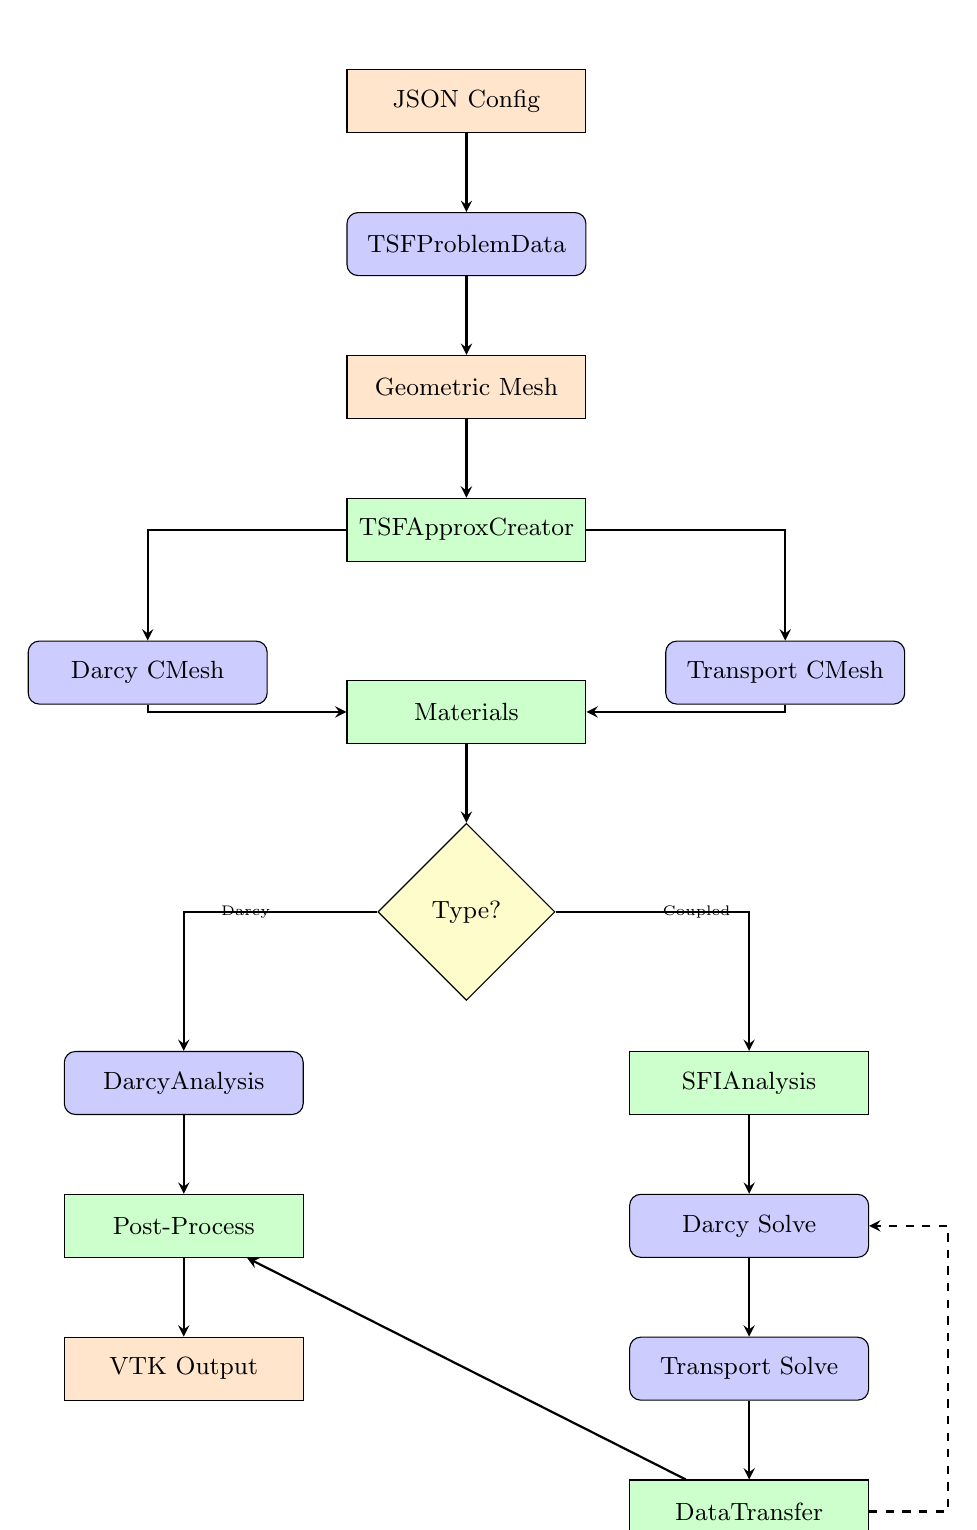
\begin{tikzpicture}[
    node distance=1.3cm,
    box/.style={rectangle, draw, fill=blue!20, text width=2.8cm, text centered, rounded corners, minimum height=0.8cm, font=\small},
    process/.style={rectangle, draw, fill=green!20, text width=2.8cm, text centered, minimum height=0.8cm, font=\small},
    decision/.style={diamond, draw, fill=yellow!20, text width=1.5cm, text centered, font=\small},
    io/.style={rectangle, draw, fill=orange!20, text width=2.8cm, text centered, minimum height=0.8cm, font=\small},
    arrow/.style={->, >=stealth, thick}
]

% Start
\node[io] (start) {JSON Config};
\node[box, below=1cm of start] (problemdata) {TSFProblemData};
\node[io, below=1cm of problemdata] (mesh) {Geometric Mesh};

% Approximation Space Creation
\node[process, below=1cm of mesh] (approx) {TSFApproxCreator};
\node[box, below left=1cm and 1cm of approx] (darcycmesh) {Darcy CMesh};
\node[box, below right=1cm and 1cm of approx] (transportcmesh) {Transport CMesh};

% Material Assignment
\node[process, below=1.5cm of approx] (materials) {Materials};

% Analysis Type Decision
\node[decision, below=1cm of materials] (analysistype) {Type?};
\node[box, below left=1.2cm and 1.5cm of analysistype] (darcy) {DarcyAnalysis};
\node[process, below right=1.2cm and 1.5cm of analysistype] (sfi) {SFIAnalysis};

% SFI components
\node[box, below=1cm of sfi] (darcysolve) {Darcy Solve};
\node[box, below=1cm of darcysolve] (transportsolve) {Transport Solve};
\node[process, below=1cm of transportsolve] (transfer) {DataTransfer};

% Post-processing
\node[process, below=1cm of darcy] (postproc) {Post-Process};
\node[io, below=1cm of postproc] (output) {VTK Output};

% Arrows - Main flow
\draw[arrow] (start) -- (problemdata);
\draw[arrow] (problemdata) -- (mesh);
\draw[arrow] (mesh) -- (approx);
\draw[arrow] (approx) -| (darcycmesh);
\draw[arrow] (approx) -| (transportcmesh);
\draw[arrow] (darcycmesh) |- (materials);
\draw[arrow] (transportcmesh) |- (materials);
\draw[arrow] (materials) -- (analysistype);

% Decision branches
\draw[arrow] (analysistype) -| node[near start, left, font=\tiny] {Darcy} (darcy);
\draw[arrow] (analysistype) -| node[near start, right, font=\tiny] {Coupled} (sfi);

% Darcy path
\draw[arrow] (darcy) -- (postproc);

% SFI path
\draw[arrow] (sfi) -- (darcysolve);
\draw[arrow] (darcysolve) -- (transportsolve);
\draw[arrow] (transportsolve) -- (transfer);
\draw[arrow] (transfer) -- (postproc);

% Loop back
\draw[arrow, dashed] (transfer.east) -- ++(1,0) |- (darcysolve.east);

% Post-processing
\draw[arrow] (postproc) -- (output);

\end{tikzpicture}
}
\caption{Complete workflow for multiphase flow simulation with subFlow}
\end{figure}

\subsection{Data Transfer and Coupling Mechanism}

\begin{figure}[h]
\centering
\scalebox{0.8}{
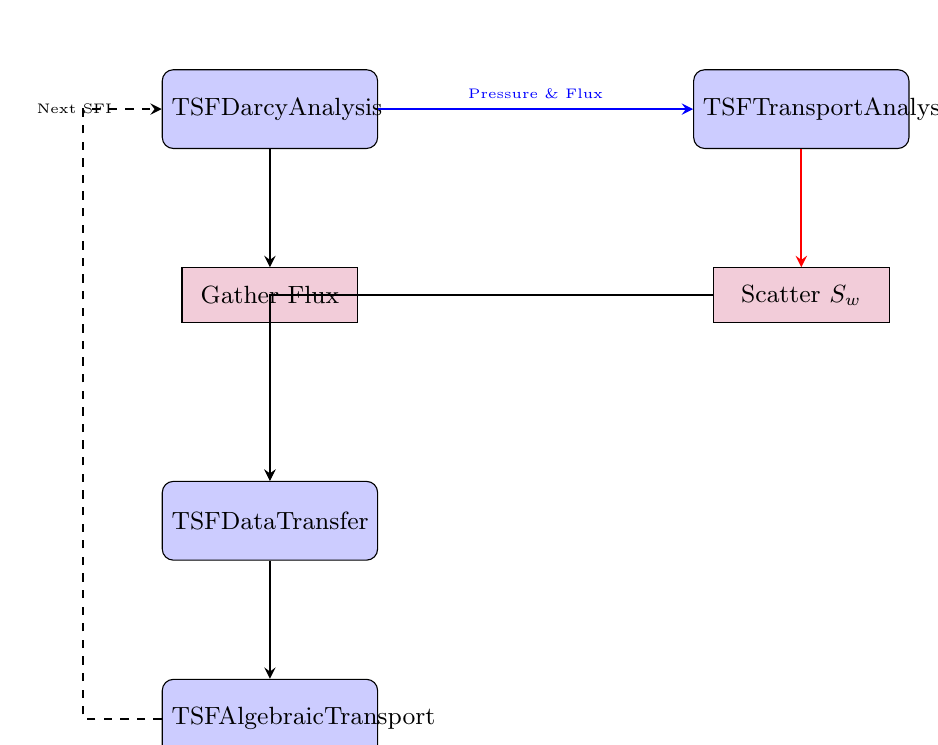
\begin{tikzpicture}[
    node distance=2cm,
    box/.style={rectangle, draw, fill=blue!20, text width=2.5cm, text centered, rounded corners, minimum height=1cm, font=\small},
    transfer/.style={rectangle, draw, fill=purple!20, text width=2cm, text centered, minimum height=0.7cm, font=\small},
    arrow/.style={->, >=stealth, thick}
]

\node[box] (darcy) {TSFDarcyAnalysis};
\node[box, right=4cm of darcy] (transport) {TSFTransportAnalysis};

% Data Transfer Components
\node[transfer, below=1.5cm of darcy] (gather) {Gather Flux};
\node[transfer, below=1.5cm of transport] (scatter) {Scatter $S_w$};
\node[box, below=2cm of gather] (datatransfer) {TSFDataTransfer};
\node[box, below=1.5cm of datatransfer] (algebraic) {TSFAlgebraicTransport};

% Forward arrows (Darcy to Transport)
\draw[arrow, blue] (darcy) -- node[above, font=\tiny] {Pressure \& Flux} (transport);
\draw[arrow] (darcy) -- (gather);
\draw[arrow] (gather) -| (datatransfer);

% Backward arrows (Transport to Darcy)
\draw[arrow, red] (transport) -- (scatter);
\draw[arrow] (scatter) -| (datatransfer);

% Central transfer hub
\draw[arrow] (datatransfer) -- (algebraic);
\draw[arrow, dashed] (algebraic.west) -- ++(-1,0) |- node[near end, left, font=\tiny] {Next SFI} (darcy.west);

\end{tikzpicture}
}
\caption{Data transfer mechanism in SFI coupling}
\end{figure}

\newpage
\section{Typical Usage Workflow}

This section demonstrates how to use the subFlow library for a coupled simulation.

\subsection{Basic Simulation Steps}

\begin{lstlisting}[language=C++]
// 1. Load problem data from JSON configuration
TSFProblemData simData;
simData.ReadJSONFile("simulation_config.json");

// 2. Build or load geometric mesh
TPZGeoMesh *gmesh = new TPZGeoMesh();
// ... populate gmesh from GMSH file or generated mesh ...

// 3. Create approximation spaces
TSFApproxCreator approxCreator(gmesh);
approxCreator.SetProblemData(&simData);
approxCreator.ConfigureDarcySpace();
approxCreator.AddDarcyMaterials();
TPZMultiphysicsCompMesh *darcy_cmesh = 
    approxCreator.CreateApproximationSpace();

// 4. Choose analysis type based on configuration
if (simData.fTNumerics.fAnalysisType == 0) {
    // Darcy problem only
    TSFDarcyAnalysis darcyAnalysis(darcy_cmesh);
    darcyAnalysis.SetProblemData(&simData);
    darcyAnalysis.Initialize();
    darcyAnalysis.RunTimeStep();
    darcyAnalysis.PostProcessTimeStep(
        gmesh->Dimension(), 0);
} else {
    // Coupled Darcy-Transport problem
    approxCreator.BuildTransportCmesh();
    TPZCompMesh *transport_cmesh = 
        approxCreator.GetTransportCmesh();
    
    // Create coupled SFI solver
    TSFSFIAnalysis sfiAnalysis(
        darcy_cmesh, transport_cmesh);
    sfiAnalysis.SetProblemData(&simData);
    sfiAnalysis.Initialize();
    sfiAnalysis.Run();  // Run complete simulation
    
    delete transport_cmesh;
}

// 5. Cleanup
delete darcy_cmesh;
delete gmesh;
\end{lstlisting}

\subsection{Configuration File Example}

A minimal JSON configuration for a coupled 2D simulation:

\begin{lstlisting}[language=json]
{
    "UseGMsh": true,
    "MshFile": "reservoir_2d.msh",
    "Dimension": 2,
    "Domains": [{
        "name": "reservoir",
        "matid": 1,
        "K": 1e-4,
        "phi": 0.25
    }],
    "Boundary": [
        {
            "name": "inlet",
            "matid": 10,
            "type": 0,
            "value": 100.0,
            "functionID": 0,
            "ExternalSaturation": 0.8,
            "SaturationFunctionID": 0
        },
        {
            "name": "outlet",
            "matid": 11,
            "type": 0,
            "value": 0.0,
            "functionID": 0,
            "ExternalSaturation": 0.0,
            "SaturationFunctionID": 0
        }
    ],
    "Numerics": {
        "AnalysisType": 2,
        "FluxOrder": 1,
        "DeltaT": 0.01,
        "NSteps": 50,
        "Gravity": [0.0, -9.81, 0.0],
        "IsAxisymmetric": false,
        "IsLinearTrace": false,
        "FourApproxSpaces": true,
        "NThreadsDarcy": 0,
        "MaxIterSFI": 5,
        "TolSFI": 1e-6,
        "MaxIterDarcy": 10,
        "ResTolDarcy": 1e-6,
        "CorrTolDarcy": 1e-6,
        "MaxIterTransport": 10,
        "ResTolTransport": 1e-6,
        "CorrTolTransport": 1e-6
    },
    "FluidProperties": {
        "WaterDensity": 1000.0,
        "WaterViscosity": 1e-3,
        "WaterCompressibility": 0.0,
        "GasDensity": 1.0,
        "GasViscosity": 1e-5,
        "GasCompressibility": 0.0,
        "DensityModel": 0,
        "ReferencePressure": 0.0
    },
    "PetroPhysics": {
        "KrModel": 0,
        "Swr": 0.0,
        "Sgr": 0.0
    },
    "ReservoirProperties": {
        "s0": {"functionType": 0, "value": 0.0},
        "p0": {"functionType": 0, "value": 0.0}
    },
    "PostProcess": {
        "PostProcessFrequency": 1,
        "NThreads": 0,
        "VTKResolution": 0
    }
}
\end{lstlisting}

\newpage
\section{Post-Processing and Output}

\subsection{VTK Output}

The library generates VTK-format output files for visualization in ParaView or other visualization tools.

\subsubsection{Available Outputs}

\begin{itemize}
    \item \textbf{Geometric Mesh:} \lstinline|gmesh-*.vtk| - Visualization of computational mesh before and after interface insertion
    \item \textbf{Darcy Solution:} \lstinline|darcy-cmesh.vtk| - Pressure and flux fields
    \item \textbf{Transport Solution:} \lstinline|transport-cmesh.vtk| - Saturation fields
    \item \textbf{Time Series:} Multiple files with step number for transient simulations
\end{itemize}

\subsubsection{Post-Processing Frequency}

Control output frequency via the JSON configuration:

\begin{lstlisting}[language=json]
"PostProcess": {
    "PostProcessFrequency": 5,  // Write output every 5 steps
    "NThreads": 0,
    "VTKResolution": 0
}
\end{lstlisting}

\subsection{Solution Variables}

The post-processing methods generate various solution fields depending on the problem type.

\subsubsection{Darcy Problem Variables}

\begin{itemize}
    \item Pressure field
    \item Total flux magnitude and components
    \item Velocity field
    \item Permeability
\end{itemize}

\subsubsection{Transport Problem Variables}

\begin{itemize}
    \item Water saturation
    \item Gas saturation
    \item Fluid density
    \item Relative permeabilities (water and gas)
    \item Fractional flows
\end{itemize}

\newpage
\section{Advanced Features}

\subsection{Axisymmetric Formulations}

For cylindrical symmetry problems, enable axisymmetric mode:

\begin{lstlisting}[language=json]
"Numerics": {
    "IsAxisymmetric": true,
    ...
}
\end{lstlisting}

The Darcy and transport solvers will automatically adjust weak forms and integration for axisymmetric geometry.

\subsection{Four-Space Mixed Formulation}

The four-space mixed formulation includes an additional space of Lagrange multipliers for improved robustness:

\begin{lstlisting}[language=json]
"Numerics": {
    "FourApproxSpaces": true,
    ...
}
\end{lstlisting}

This is enabled via static condensation in \lstinline|TSFApproxCreator::CondenseElements()|.

\subsection{Compressible Fluids}

For compressible fluids, set non-zero compressibilities in the JSON:

\begin{lstlisting}[language=json]
"FluidProperties": {
    "WaterCompressibility": 1e-9,
    "GasCompressibility": 0.01,
    "DensityModel": 0,  // Linear model
    "ReferencePressure": 101325.0
}
\end{lstlisting}

Density variations with pressure require Newton iterations in the Darcy solver.

The library supports two compressibility models for fluid density:

\textbf{Linear Density Model ($\text{DensityModel} = 0$):}
$$\rho(p) = \rho_{\text{ref}} \left[1 + c(p - p_{\text{ref}})\right]$$

where:
\begin{itemize}
    \item $\rho(p)$ is the fluid density at pressure $p$
    \item $\rho_{\text{ref}}$ is the reference density (WaterDensity or GasDensity)
    \item $c$ is the compressibility coefficient (WaterCompressibility or GasCompressibility)
    \item $p_{\text{ref}}$ is the reference pressure (ReferencePressure)
\end{itemize}

\textbf{Exponential Density Model ($\text{DensityModel} = 1$):}
$$\rho(p) = \rho_{\text{ref}} \exp\left[c(p - p_{\text{ref}})\right]$$

For incompressible fluids, set $c = 0$ to obtain constant density $\rho(p) = \rho_{\text{ref}}$.

\subsection{Relative Permeability Models}

Control the phase relative permeability computation:

\begin{lstlisting}[language=json]
"PetroPhysics": {
    "KrModel": 0,   // 0: Linear, 1: Quadratic
    "Swr": 0.1,     // Residual water saturation
    "Sgr": 0.05     // Residual gas saturation
}
\end{lstlisting}

The library supports two relative permeability models for both water and gas phases:

\textbf{Linear Model ($\text{KrModel} = 0$):}

Water relative permeability:
$$k_{r,w}(S_w) = \begin{cases}
0 & \text{if } S_w \leq S_{wr} \\
\frac{S_w - S_{wr}}{1 - S_{wr}} & \text{if } S_w > S_{wr}
\end{cases}$$

Gas relative permeability:
$$k_{r,g}(S_w) = \begin{cases}
0 & \text{if } S_g \leq S_{gr} \\
\frac{S_g - S_{gr}}{1 - S_{gr}} & \text{if } S_g > S_{gr}
\end{cases}$$

where $S_g = 1 - S_w$ is the gas saturation.

\textbf{Quadratic Model ($\text{KrModel} = 1$):}

Water relative permeability:
$$k_{r,w}(S_w) = \begin{cases}
0 & \text{if } S_w \leq S_{wr} \\
\left(\frac{S_w - S_{wr}}{1 - S_{wr}}\right)^2 & \text{if } S_w > S_{wr}
\end{cases}$$

Gas relative permeability:
$$k_{r,g}(S_w) = \begin{cases}
0 & \text{if } S_g \leq S_{gr} \\
\left(\frac{S_g - S_{gr}}{1 - S_{gr}}\right)^2 & \text{if } S_g > S_{gr}
\end{cases}$$

where:
\begin{itemize}
    \item $k_{r,w}(S_w)$ is the water relative permeability
    \item $k_{r,g}(S_w)$ is the gas relative permeability
    \item $S_w$ is the water saturation
    \item $S_g = 1 - S_w$ is the gas saturation
    \item $S_{wr}$ is the residual water saturation (Swr)
    \item $S_{gr}$ is the residual gas saturation (Sgr)
\end{itemize}

\end{document}
